\part{Design}
\label{part:design}

\begin{frame}[fragile]{Ansatz -- Magnetfeld}
\begin{itemize}
\item Magnetfeld als räumlich in die Spule eingebettete, dreidimensionale Geometrie anzeigen
\item Zwei verschiedene schematische Darstellungen für Magnetfeld anbieten: Vektor-Modell und Feldlinien-Modell
\item Einbettung durch Depth Cues unterstützen (in erster Linie Verdeckung der virtuellen Geometrie durch reale Spule)
\item Sensordaten in Echtzeit an HoloLens übermitteln und Geometrie auf dem Device in Echtzeit berechnen und darstellen
\end{itemize}
\end{frame}

\begin{frame}
\vspace{-1em}
\begin{center}
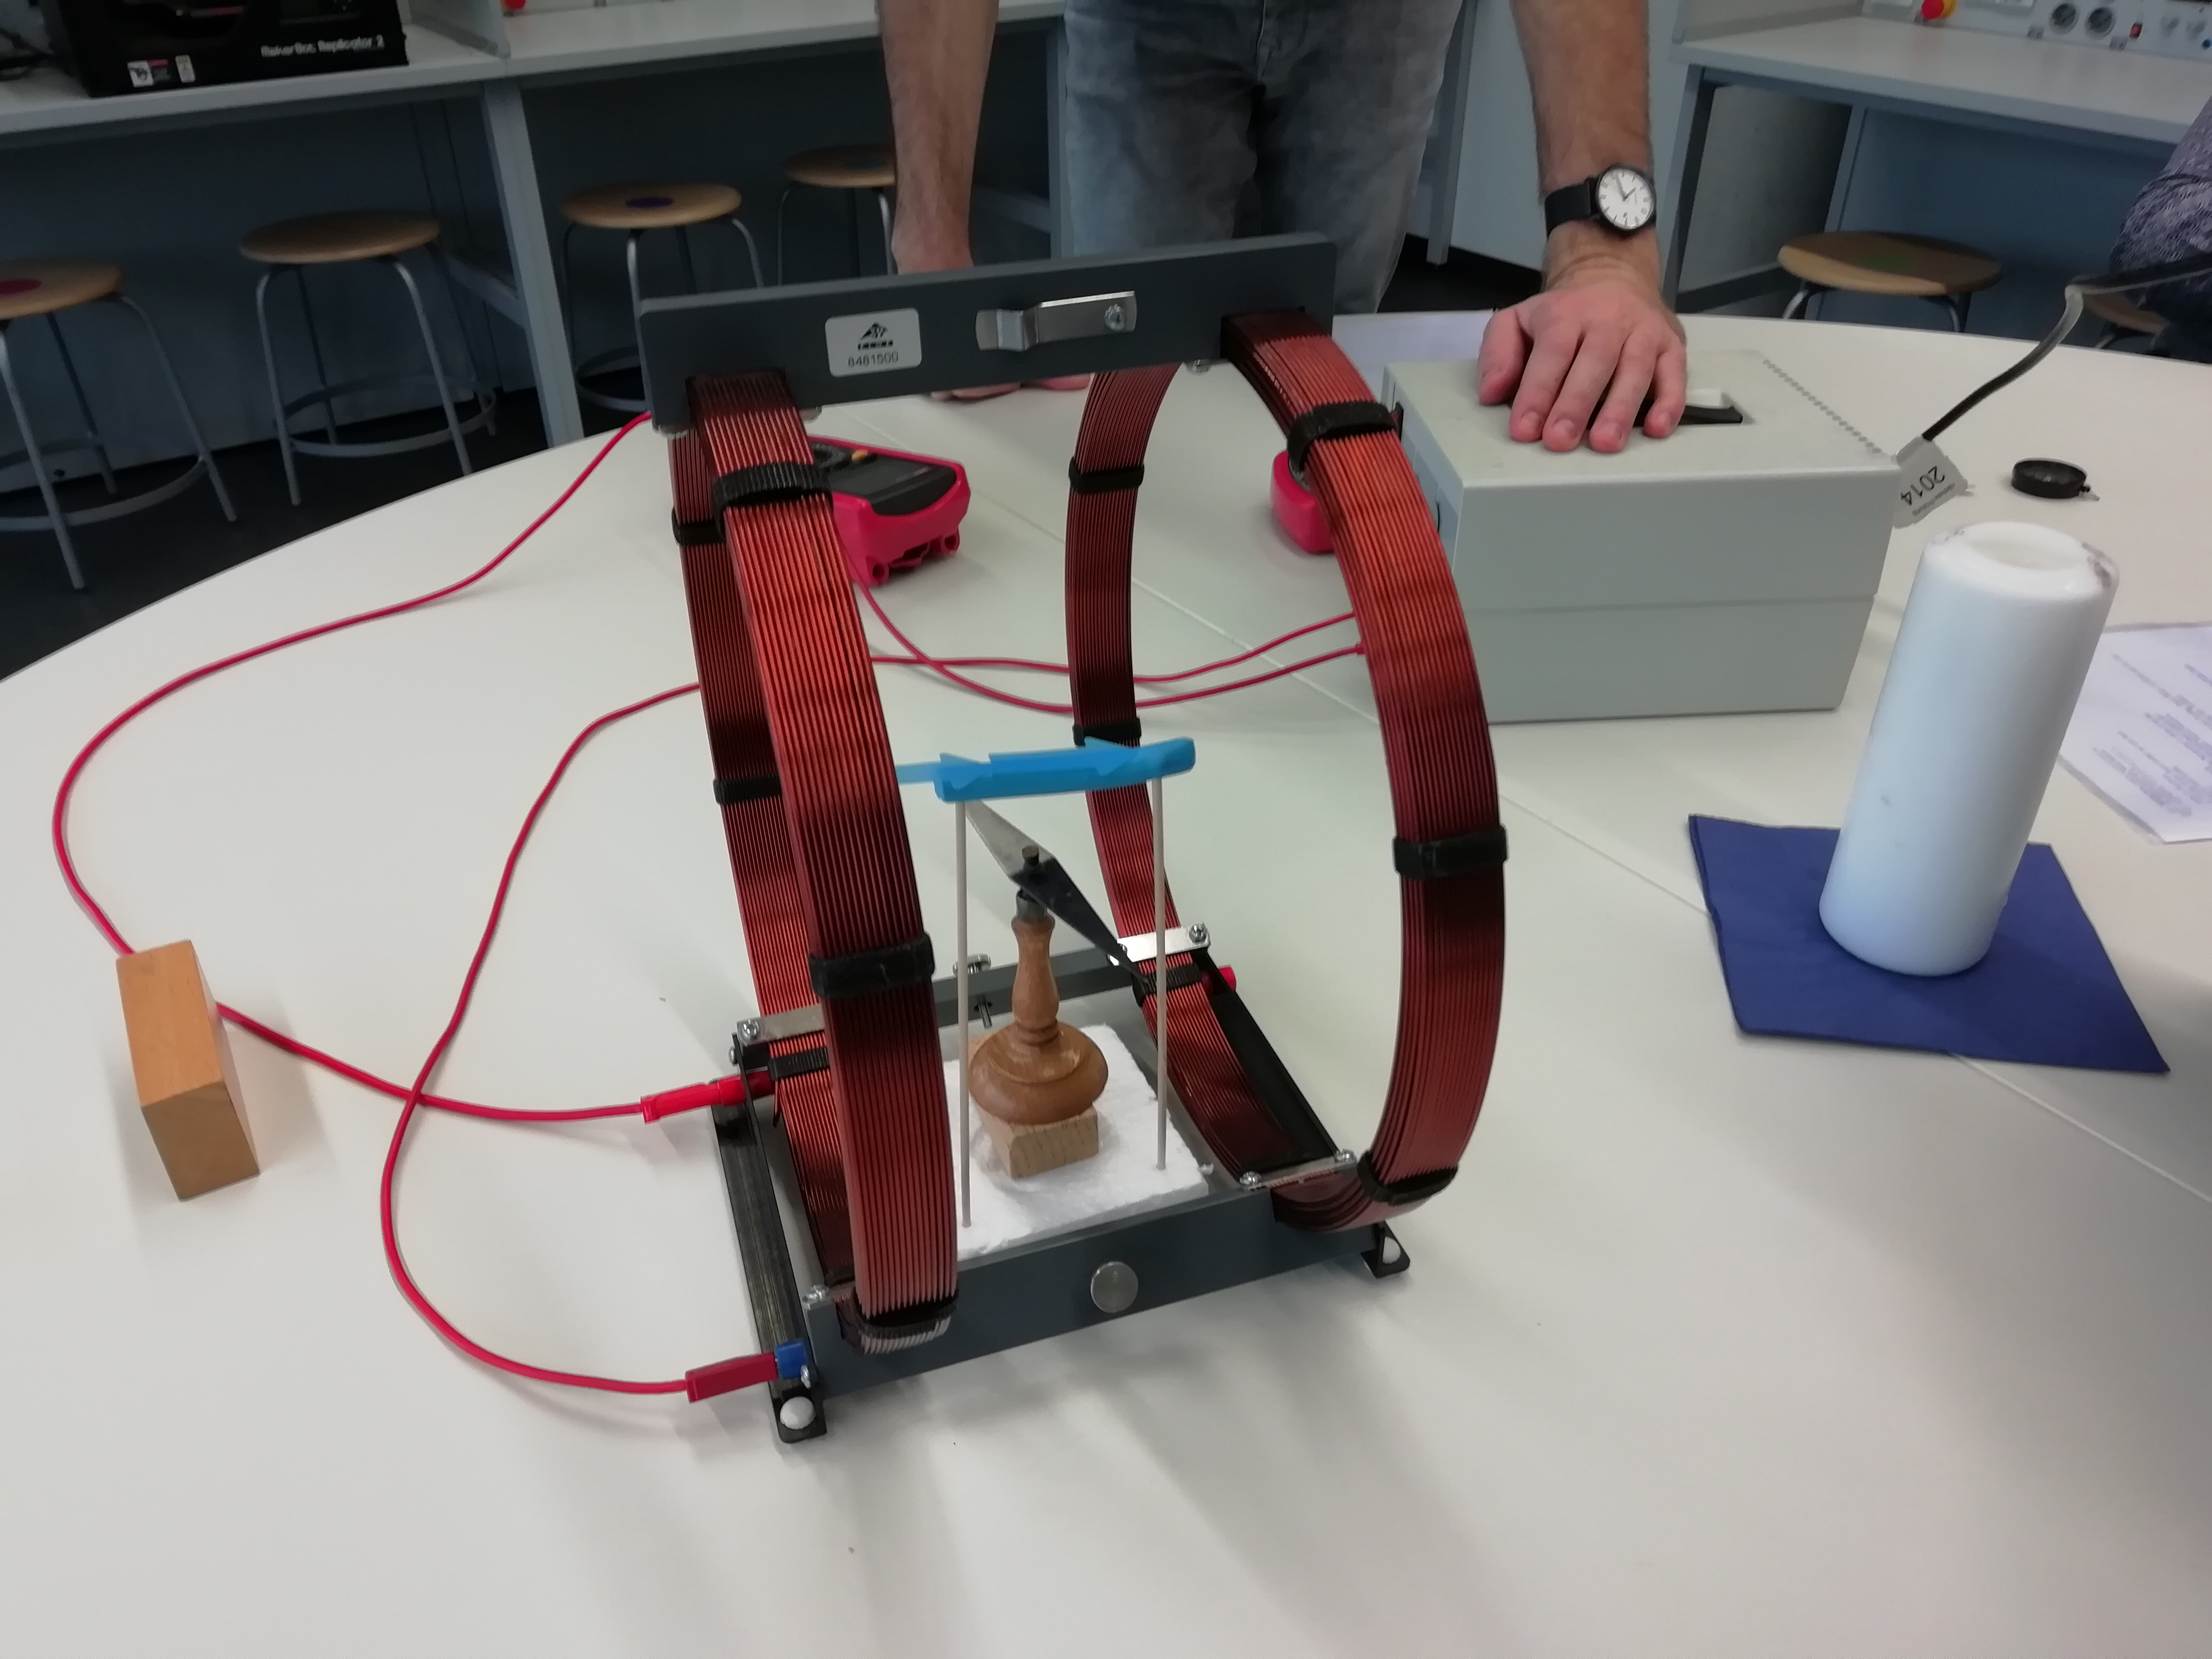
\includegraphics[width=0.8\textwidth]{images/Design_Magnetfeld.jpg}	
\end{center}
\end{frame}

\begin{frame}[fragile]{Vergleich mit Anforderungen}
\begin{itemize}
\item Inhaltliche Anforderungen
\item Distanz, Geschwindigkeit, Farbe von Objekten
\item Keine Störung der Sensorik
\item Keine Störung der Sensorik	

\item Einbettung durch Depth Cues unterstützen (in erster Linie Verdeckung der virtuellen Geometrie durch reale Spule)
\item Sensordaten in Echtzeit an HoloLens übermitteln und Geometrie auf dem Device in Echtzeit berechnen und darstellen
\end{itemize}
\end{frame}

\begin{frame}[fragile]{Ansatz -- Weitere Elemente }
\begin{itemize}
\item Eingebetteter 3D-Kompass mit Markierungen anzeigen
\item Statusinformationen als Text-UI Elemente anzeigen
\item Stromfluss durch 2D Geometrie, verankert an den beiden Spulen-Teilen, visualisieren
\end{itemize}
\end{frame}


\part{Umsetzung und Ausblick}
\label{part:practice}

\begin{frame}[fragile]{}
asdf
\end{frame}